\subsection{Аффинный шифр}

Аффинный шифр --- это частный случай более общего моноалфавитного шифра 
подстановки. К шифрам подстановки относятся также шифр Цезаря, 
ROT13 и Атбаш. Поскольку аффинный шифр легко дешифровать, 
он обладает слабыми криптографическими свойствами.

\subsubsection{Описание аффинного шифра}

В аффинном шифре каждой букве алфавита размера m ставится в 
соответствие число из диапазона $[0, ..., m - 1]$. 
Затем при помощи модульной арифметики для каждого числа, соответствующего 
букве исходного алфавита, вычисляется новое число, которое заменит 
старое в шифротексте. Функция шифрования для каждой буквы

    $$\mbox{E}(x) = (ax + b) \mod{m},$$

где модуль $m$ --- размер алфавита, а пара $a$ и $b$ --- ключ шифра. Значение 
$a$ должно быть выбрано таким, что $a$ и $m$ --- 
взаимно простые числа. Функция 
расшифрования

    $$\mbox{D}(x) = a^{-1} \times (x - b) \mod{m},$$

где $a^{-1}$ --- обратное к $a$ число по модулю $m$. 
То есть оно удовлетворяет уравнению

    $$1 \equiv a \times a^{-1} \mod{m}.$$

Обратное к $a$ число существует только в том случае, когда 
$a$ и $m$ --- взаимно 
простые. Значит, при отсутствии ограничений на выбор числа $a$ 
расшифрование 
может оказаться невозможным. Покажем, что функция расшифрования является 
обратной к функции шифрования:

$$\begin{matrix}
    \mbox{D}(\mbox{E}(x)) 
      &= &a^{-1} \times (\mbox{E}(x) - b) \mod{m} \\ 
      &= &a^{-1} \times ((ax + b) - b) \mod{m} \\ 
      &= &a^{-1} \times (ax + b - b) \mod{m} \\ 
      &= &a^{-1} \times ax \mod{m}\\ 
      &= &x \mod{m}. 
\end{matrix}$$

Количество возможных ключей для аффинного шифра можно записать 
с помощью функции Эйлера как $\varphi(m) \times m$.

\subsubsection{Криптоанализ, минимизация вариантов перебора}

Так как аффинный шифр является по сути моноалфавитным шифром замены
, то он обладает всеми уязвимостями этого класса шифров. Шифр Цезаря —
это аффинный шифр с $a = 1$, что сводит функцию шифрования к простому 
линейному сдвигу.

В случае шифрования сообщений на русском языке (т. е. с помощью $m = 33$) 
существует 627 нетривиальных аффинных шифров, не учитывая 33 тривиальных шифра 
Цезаря. Это число легко посчитать, зная, что существует всего 20 чисел 
взаимно простых с 33 и меньших 33 (а это и есть возможные значения 
$a$). Каждому значению a могут соответствовать 33 разных дополнительных 
сдвига (значение $b$); то есть всего существует 2033 или 660 возможных 
ключей. Аналогично, для сообщений на английском языке (т.е. $m = 26$) 
всего существует 1226 или 312 возможных ключей. Такое ограниченное 
количество ключей приводит к тому, что система крайне не криптостойка 
с точки зрения принципа Керкгоффса.

Основная уязвимость шифра заключается в том, что криптоаналитик может 
выяснить (путем частотного анализа, полного перебора, угадывания или 
каким-либо другим способом) соответствие между двумя любыми буквами 
исходного текста и шифротекста. Тогда ключ может быть найдет путем 
решения системы уравнений. Кроме того, так мы знаем, что $a$ и $m$ — взаимно 
простые, это позволяет уменьшить количество проверяемых ключей для 
полного перебора:

\begin{figure}[bh]
\noindent\centering{
    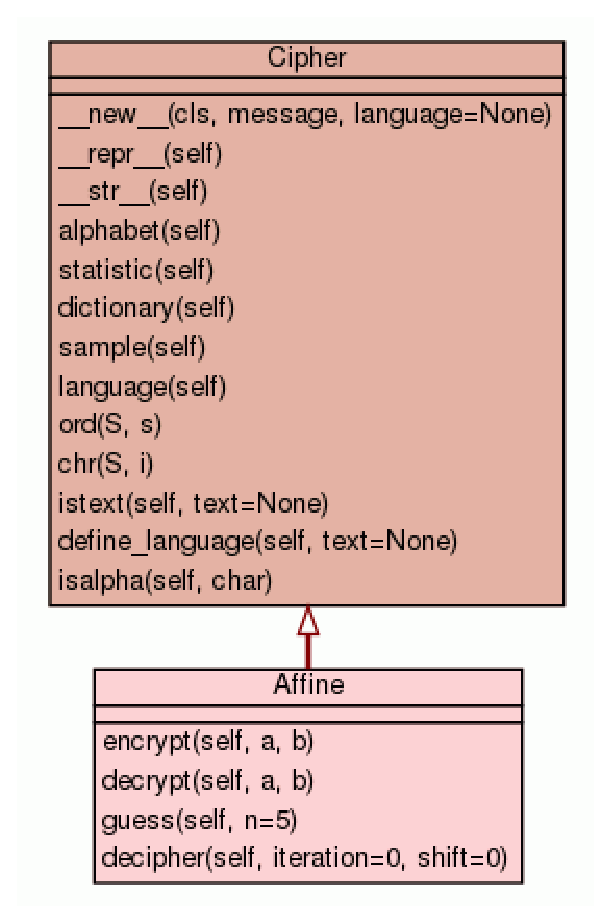
\includegraphics[width=65mm]{\globalImages/uml_affine.eps}
}
\caption{UML диаграмма класса анализа афинного шифра}
\label{figCurves}
\end{figure}

\begin{listing}[1]{1}
def decipher(self, iteration = 0, shift = 0):
    base = range(1, len(self.alphabet) + 1)
    for a in base:
        coprimes = [b for b in base if cipher.routine.gcd(a, b) == 1]
        for b in coprimes:
            ot = self.decrypt(a, b)
            if self.istext(ot) > 0.7:
                return (ot, a, b)
\end{listing}

Преобразование, подобное аффинному шифру, используется в линейном 
конгруэнтном методе (разновидности генератора псевдослучайных чисел).
Этот метод не является криптостойким по той же причине, что и аффинный 
шифр.

Диаграмма показывает, что афинный шифр успено вписывается 
в разработанную архитектуру.
